\subsection{Correlating Microarchitecture with Performance\jled{change to ``Benchmarking''?}}
\label{sec:benchmark}


To explore NVIDIA Kepler architecture, we a create microbenchmark tailored for each considered characteristic.
% Our following observations are drawn from analyzing the execution time of the microbenchmarks.
Each program from the microbenchmark is basically a main function of CUDA kernel code with timing around.
Timing ticks are recorded in a general register by reading the clock register (using clock()) and then time is calculated and written to global memory.
% The clock values are
% first stored in registers, then written to global memory at the
% end of the kernel to avoid slow global memory accesses from
% interfering with the timing measurements.
For timing accuracy, the same CUDA kernel code is duplicated for several times and the average time is used for analysis.
% The general structure of a microbenchmark consists of GPU
% kernel code containing timing code around a code section (typically an unrolled loop running multiple times) that exercises
% the hardware being measured. 
We run each benchmark program twice, disregarding the first run to avoid compulsory instruction cache misses. 
We make sure that all CUDA kernel codes are small enough to fit into the L1 instruction cache.
The throughput is the maximum number of instructions of the same kind that can being executed per clock
cycle when the operands of each instruction are independent of the preceding instructions.
We use similar test method as~\cite{fog}.

By comparing the execution time of each inside program, we get the following observations.

With the assembler we tune the assembly codes of microbenchmark. According to the performance tuning results, we 
correlate microarchitecture with performance variants that guide optimizations in real applications. The correlation is 
presented as several meaningful observations, which are categorized into four microarchitectural features:  {\tt 
control} function, {\tt register} allocation, {\tt arithmetic} throughput and {\tt memory} operation.
    \begin{figure*}
        \begin{subfigure}[htbp]{0.3\textwidth}
            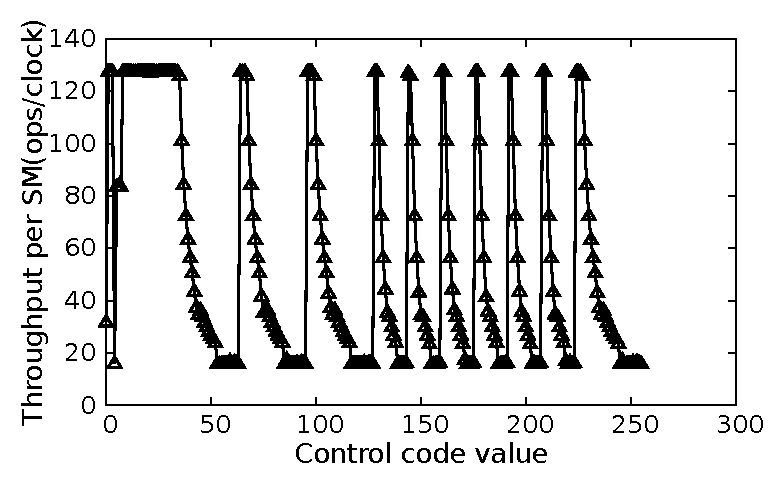
\includegraphics[width=2.1in]{ctrl}
           \subcaption{Regulate {\tt FFMA} throughput.}
            \label{fig:control_throughput}
        \end{subfigure}
        \begin{subfigure}[htbp]{0.3\textwidth}
            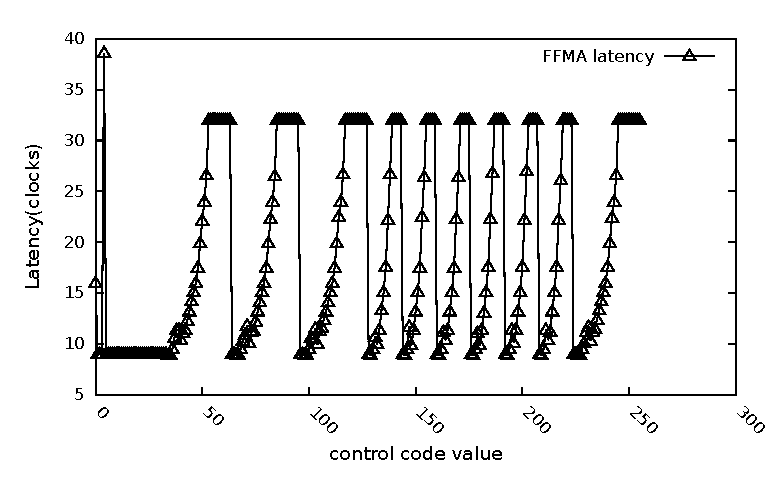
\includegraphics[width=2.1in]{ctrl_latency}
            \subcaption{Regulate {\tt FFMA} latency.}
            \label{fig:control_latency}
        \end{subfigure}
        \begin{subfigure}[htbp]{0.3\textwidth}
            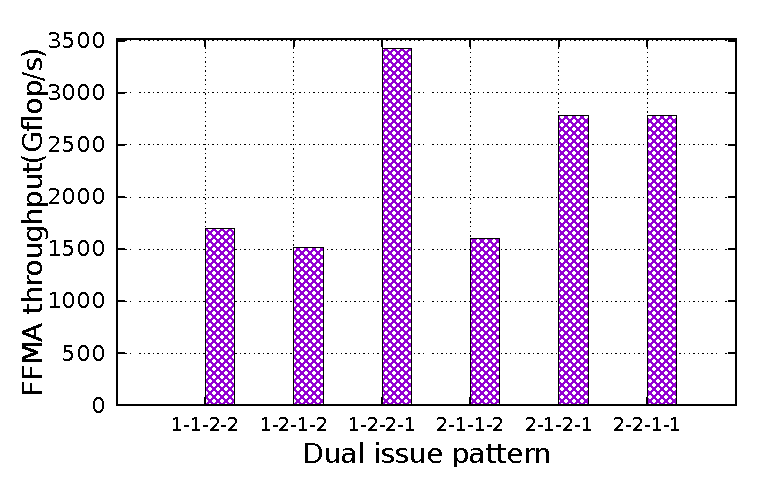
\includegraphics[width=2.1in]{pattern}
            \subcaption{Peak {\tt FFMA} throughput(S:single issue, D:dual issue).}
            \label{fig:control_pattern}
        \end{subfigure}
        \caption{Different control code impact on performance}\label{fig:control_code}
    \end{figure*}


{\em {\bf Observation 1--[Control]}: The execution sequence of instructions is regulated by control codes. Both warp 
scheduling and issue mode are tunable by setting control codes.}

Starting with the Kepler architecture, NVIDIA has been moving some control logic off the chip and into kernel 
instructions which are determined by the assembler~\cite{lai,maxas}. This evolution provides programmer a chance to 
make globally optimal decisions on scheduling and other control aspects if an assembler is available. The disassembly 
code on Figure~\ref{fig:assemblycode} shows that on Kepler control code is placed before seven instructions, and it 
indicates that every $64$ bits control code controls $7$ instructions. We identify that both higher $6$ bits and lower 
$2$ bits are {\em opcode} of control code, and the middle $56$ bits are used to control the execution of $7$ 
instructions, each of which is assigned $8$ control bits.

For the eight control bits, we identify their meanings by statically examining CUBLAS disassembly codes of CUBLAS and 
dynamically benchmarking instruction sequence of different control codes. We observe that the $7$th bit of the control 
code of {\tt TEXDEPBAR} instruction is $1$, which
indicates a texture dependency barrier due to weak consistent memory model of texture cache. It's verified that some 
unexpected values are
loaded if this bit is not set. Similarly, we discover that the $5$th bit means shared memory dependency barrier, the
$4$th bit means global memory dependency barrier. Figure~\ref{fig:control_code}(\subref{fig:control_throughput}) and 
Figure~\ref{fig:control_code}(\subref{fig:control_latency}) shows that {\tt FFMA} throughput and latency varies with 
all control bit values from 0 to 255. As shown in this figure, the throughput linearly decreases with the increasing 
values represented by the $0-3$ bits. That implies that these $4$ bits set the number of stall cycles before issuing 
the instruction. Further, the microbenchmarking reveals some specific patterns of control codes:

\begin{itemize}
\item When the control bits are set to be $0x00$, the scheduler suspends a warp of the instructions for $16$ cycles.
\item $0x20|n$ means a warp is suspended for $n$ cycles before issuing the next instruction, where $n$ is number 
between $0$ and $15$.
\item $0x04$ means dual issue mode. If two consecutive instructions is controlled by $0x04$ and $0x05$, the throughput 
can reach the maximum. Single issue control code is $0x00$.
\end{itemize}


{\em {\bf Observation 2--[Register]}: Irrespective of single- or dual-issue mode, register bank conflict is only caused 
by source operands, and degrades instruction throughput.}

For CUDA programming model it is well-known that shared memory bank conflict is an important performance factor. In
fact, recent research~\cite{lai} noticed that register bank conflicts are nontrivial to performance.  In order to probe 
register bank conflict, our microbenchmark measures instruction throughput for different combination of {\tt FFMA} 
register operands. Table~\ref{tab:th} shows an example of the combination which results in variance of efficiency. The 
numbers in the fifth column represent the number of registers conflicts in the same bank. This experiment is conducted 
in single-issue mode by setting control code to be $0x20$. The theoretical efficiency is $128/192=66.67\%$. In fact, we 
observe that both single- and dual-issue mode produce the same variance of instruction throughput. Besides, from the 
experimental results we observe that:
\begin{itemize}
\item Destination operand will not contribute to bank conflict, no matter which bank is assigned to it.
\item When source operands have 2-way conflict, the throughput will drop by 2.33\% in single issue
    mode. When source operands have 3-way conflicts, the throughput will drop by up to 17.17\%.

 \item On Kepler architecture, our microbenchmark finds out a proper distribution of registers for eliminating bank
     conflict. The distribution is summarized in Table~\ref{tab:reg}, which confirms the rule~\cite{lai}: \\
 bank0$\Leftarrow$($Rindex \% 8 < 4$ \&\& $Rindex \% 2 == 0$) \\
 bank2$\Leftarrow$($Rindex \% 8 < 4$ \&\&
$Rindex \% 2 == 1$) \\
bank1$\Leftarrow$($Rindex \% 8 > 4$ \&\& $Rindex \%2 == 0$) \\
bank3$\Leftarrow$($Rindex \% 8 < 4$ \&\&
$Rindex\% 2 == 1$)\\
where $Rindex$ is the register number. This rule will guide the performance tuning in the following SGEMM 
implementation.

\end{itemize}

\begin{table}[htbp]
    \caption{The efficiency of instruction throughput varies with difference register bank distribution. {\it Inst} : 
instruction pattern, {\it Th/SM}: the instruction throughput per SM, {\it Eff}: efficiency of throughput, {\tt Conf} 
register bank conflicts.}
\centering
\scalebox{1.0} {
\begin{tabular}{|c|c|c|c|}
\hline
Inst &Th/SM&Eff&Conf\\
\hline
{\tt FFMA R5,R4,R1,R0}&127.50&66.40\%&0\\
\hline
{\tt FFMA R2,R4,R1,R0}&127.50&66.40\%&0\\
\hline
{\tt FFMA R5,R2,R1,R0}&119.18&62.07\%&2-way\\
\hline
{\tt FFMA R3,R2,R1,R0}&119.18&62.07\%&2-way\\
\hline
{\tt FFMA R5,R9,R3,R1}&94.52&49.23\%&3-way\\
\hline
{\tt FFMA R11,R9,R3,R1}&94.52&49.23\%&3-way\\
\hline
{\tt FMUL R4,R1,R0}&127.50&66.40\%&0\\
\hline
{\tt FMUL R4,R2,R0}&119.17&62.06\%&2-way\\
\hline
\end{tabular}
}
\label{tab:th}
\end{table}


\begin{table}[htbp]
\caption{Register corresponding bank.}
\centering
\scalebox{1.0} {
\begin{tabular}{|c|c|c|c|c|c|c|c|c|}
\hline
    {\tt Bank0}&{\tt R0}&{\tt R2}&{\tt R8}&{\tt R10}&{\tt R16}&{\tt R18}&{\tt R24}&{\tt R26}\\
\hline
    {\tt Bank1}&{\tt R1}&{\tt R3}&{\tt R9}&{\tt R11}&{\tt R17}&{\tt R19}&{\tt R25}&{\tt R27} \\
\hline
    {\tt Bank2}&{\tt R4}&{\tt R6}&{\tt R12}&{\tt R14}&{\tt R20}&{\tt R22}&{\tt R28}&{\tt R30}\\
\hline
    {\tt Bank3}&{\tt R5}&{\tt R7}&{\tt R13}&{\tt R15}&{\tt R21}&{\tt R23}&{\tt R29}&{\tt R31}\\
\hline
\end{tabular}
}
\label{tab:reg}
\end{table}

{\em {\bf Observation 3--[Arithmetic]}: With a proper control code pattern and register allocation, {\tt FFMA} 
instruction throughput can approach the theoretical peak in dual issue mode.}

It's very intricate to tune instruction execution to improve instruction throughput. The previous work~\cite{lai} 
report a maximal throughput of {\tt FFMA} per SM is $132$, which is much less than the theoretical throughput which is 
$192$ on Kepler. Our microbenchmarks reveal several key points of optimization to approach theoretical peak on Kepler. 
First, the control code must be set properly to dual issue adjacent instructions. Second, the ratio and interval of 
dual issue {\tt FFMA} instructions must be tuned into a specific pattern. Since each warp of extra computing unit is 
shared among two warps, when all threads are trying to fully dual issue every two adjacent {\tt FFMA}s, half of the 
scheduler would stall due to computing resource conflict. The ratio of dual issue and single issue should be $2:2$, and 
with a proper phase shift among two warp's executing pace, they could get access to the shared computing unit in turn. 
There are $C(4,2)=6$ combinations for single dual issue pattern inside a seven instructions sheduling block, which is 
shown in Figure~\ref{fig:control_code}(\subref{fig:control_pattern}). {\tt SDDS} behaves best, so we choose this 
pattern in our implementation. Third, the first instruction of the core loop needs to be aligned. This restriction is 
caused by the aligned position of control code in the instruction sequence. Last, {\tt FFMA} dual issue requires 6 
register banks. Instruction order has to be adjusted to fully use Kepler's operand 
collector~\cite{collector,tarjan2012policy} mechanism to avoid register bank conflicts. As shown in 
Table~\ref{tab:ffma}, these optimizations together improve {\tt FFMA}'s throughput  to be $190$, which is very close to 
the theoretical peak $192$.

\begin{table}[htbp]
\caption{Floating-point instruction throughput on Kepler}
\centering
\scalebox{1.} {
\begin{tabular}{|c||c|c|c|}
\hline
Inst &operation&single issue&dual issue\\
\hline
{\tt FFMA} &c=a*b+c&127.52&190.35 \\
\hline
{\tt FMUL} &c=a*b&127.52&190.35 \\
\hline
{\tt FADD} &c=a+b&127.52&191.50\\
\hline
\end{tabular}
}
\label{tab:ffma}
\end{table}


{\em {\bf Observation 4--[Memory]}: For achieving higher memory bandwidth, shared memory prefers to 64-bits load 
instruction {\tt LDS.64} while global memory prefers to load instruction {\tt LDG} with texture path.}

For the GPU memory hierarchy we focus on the programmer controllable memory resources--shared memory and global memory. 
On NVIDIA GPU architecture, there are different memory access widths (i.e., 32-bits,64-bits,128-bits) and paths (i.e., 
normal cache or texture cache). In fact, both NVIDIA document and previous works~\cite{tan} pointed out that wider 
instructions have longer pipeline latencies, which are also measured in our microbenchmark. In addition, we identify 
several bandwidth issues for memory optimization.

Intuitively, a wider load operation achieves higher bandwidth. We benchmark bandwidth of shared memory operations {\tt 
LDS} with different widths, i.e., {\tt LDS.32}, {\tt LDS.64}
and {\tt LDS.128}. The operations are specially arranged so that no shared memory bank conflict occurs in a warp. In the
experiment, the amount of data are projected to the number of load instructions. For exmaple, if the data are loaded by
$N$ {\tt LDS.128} instructions, then either $2N$ {\tt LDS.64} or $2N$ {\tt LDS.64} instructions are required.
Figure~\ref{fig:lds_bw} compares the sequential memory access bandwidth with increasing volume of data. As shown in the 
figure, {\tt LDS.64} achieves the highest bandwidth $137GB/s$, which is about $76\%$ of the peak bandwidth\footnote{The 
theoretical shared memory bandwidth for each SM can be calculated as $Bandwidth=f_{core}*Width*Warpsize$ in
bytes, where $f_{core}$ is frequency of CUDA core, $Width$ is bank width, $Warpsize$ is warp size.}.

\begin{figure}[htbp]
\begin{center}
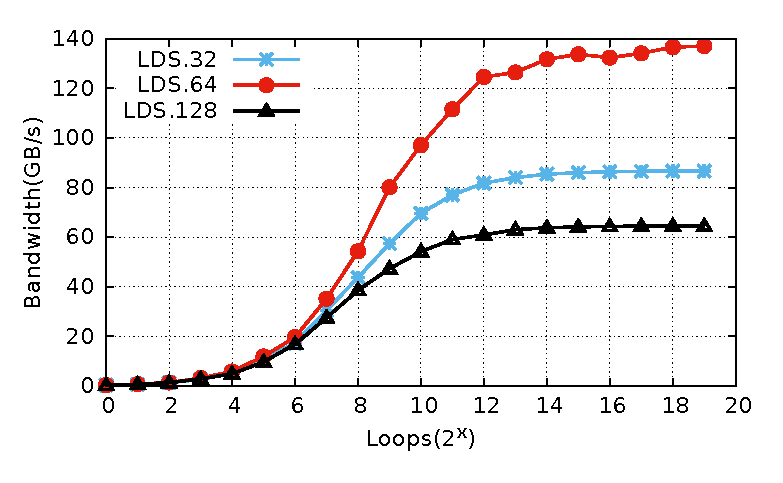
\includegraphics[scale=0.6]{lds_bandwidth}
    \caption{ Bandwidth of {\tt LDS.32}, {\tt LDS.64} and {\tt LDS.128}}
\label{fig:lds_bw}
\end{center}
\end{figure}

% global memory
There are two paths to global memory. One is from global memory to L2 cache, which is executed by {\tt
LD} instruction. The other one is from global memory to texture cache, which is executed by {\tt LDG} instruction. We
launch $26$ thread blocks with $512$ threads, and specifies that each thread access $4$ words with a stride of
$4*blockDim.x*gridDim.x$. Our benchmark confirms that {\tt LDG} achieves higher bandwidth than {\tt LD}, which has been
identified by previous work~\cite{tan}.
